\documentclass[twoside,twocolumn]{article}

\usepackage{blindtext} % Package to generate dummy text throughout this template 
\usepackage{graphicx}
\usepackage[sc]{mathpazo} % Use the Palatino font
\usepackage[T1]{fontenc} % Use 8-bit encoding that has 256 glyphs
\linespread{1.05} % Line spacing - Palatino needs more space between lines
\usepackage{microtype} % Slightly tweak font spacing for aesthetics

\usepackage[english]{babel} % Language hyphenation and typographical rules

\usepackage[hmarginratio=1:1,top=32mm,columnsep=20pt]{geometry} % Document margins
\usepackage[hang, small,labelfont=bf,up,textfont=it,up]{caption} % Custom captions under/above floats in tables or figures
\usepackage{booktabs} % Horizontal rules in tables

\usepackage{lettrine} % The lettrine is the first enlarged letter at the beginning of the text

\usepackage{enumitem} % Customized lists
\setlist[itemize]{noitemsep} % Make itemize lists more compact

\usepackage{abstract} % Allows abstract customization
\renewcommand{\abstractnamefont}{\normalfont\bfseries} % Set the "Abstract" text to bold
\renewcommand{\abstracttextfont}{\normalfont\small\itshape} % Set the abstract itself to small italic text

\usepackage{titlesec} % Allows customization of titles
\renewcommand\thesection{\Roman{section}} % Roman numerals for the sections
\renewcommand\thesubsection{\roman{subsection}} % roman numerals for subsections
\titleformat{\section}[block]{\large\scshape\centering}{\thesection.}{1em}{} % Change the look of the section titles
\titleformat{\subsection}[block]{\large}{\thesubsection.}{1em}{} % Change the look of the section titles

\usepackage{fancyhdr} % Headers and footers
\pagestyle{fancy} % All pages have headers and footers
\fancyhead{} % Blank out the default header
\fancyfoot{} % Blank out the default footer
\fancyhead[L]{Frameworks de pruebas } % Custom header text
\fancyhead[R]{November 2020 } % Custom header text
\fancyfoot[RO,LE]{\thepage} % Custom footer text

\usepackage{titling} % Customizing the title section

\usepackage{hyperref} % For hyperlinks in the PDF
\usepackage{array}
%----------------------------------------------------------------------------------------
%	TITLE SECTION
%----------------------------------------------------------------------------------------

\setlength{\droptitle}{-4\baselineskip} % Move the title up

\pretitle{\begin{center}\Huge\bfseries} % Article title formatting
\posttitle{\end{center}} % Article title closing formatting
\title{FRAMEWORKS DE PRUEBAS} % Article title
\author{Arias, Cancino, Crispin, Gutierrez, Zuñiga} 
\date{\today} % Leave empty to omit a date
\renewcommand{\maketitlehookd}{%
\begin{abstract}
	\begin{center}
		\textbf{Resumen}
	\end{center}
	La prueba de API es un tipo de prueba de software que se centra en determinar si las API cumplen con las expectativas. Dado que las API se están convirtiendo en el componente esencial del desarrollo de software, es necesario que los desarrolladores y programadores realicen pruebas de API. Esta prueba no se puede realizar en el front-end ya que no hay una interfaz gráfica de usuario para las API. A continuación, analizamos 2 herramientas de prueba de API, describiendo sus pros y contras.
\\
	\begin{center}
		
		\textbf{Abstract}
	\end{center}
	API testing is a type of software testing that focuses on determining if APIs meet expectations. As APIs are becoming the essential component of software development, API testing is required by developers and programmers. This test cannot be done on the front end as there is no graphical user interface for the APIs. Below we discuss 2 API testing tools, describing their pros and cons.
	\\
\end{abstract}
}
%----------------------------------------------------------------------------------------

\begin{document}
% Print the title
\maketitle
\vspace*{5 in}
\section{Introducción}
Las pruebas de API son un tipo de prueba de software que implica probar las interfaces de programación de aplicaciones (API) directamente y como parte de las pruebas de integración para determinar si cumplen con las expectativas de funcionalidad, confiabilidad, rendimiento y seguridad
\\
\section{Desarrollo}
\textbf{¿Qué es un cliente API?}\\
“Un cliente API es un conjunto de herramientas y protocolos que operan desde una aplicación en una computadora. Le ayudan a evitar algunas operaciones al desarrollar una aplicación web en lugar de reinventar la rueda cada vez. El uso de una API de cliente es una excelente manera de acelerar el proceso de desarrollo. “
Insomnia y Postman se conocen como clientes HTTP / API. Proporcionan una interfaz gráfica de usuario (GUI) para enviar  solicitudes HTTP .
Los clientes de API permiten a los usuarios diseñar y probar API rápidamente. En consecuencia, esto puede aumentar considerablemente la velocidad de desarrollo.


\textbf{Herramientas de prueba de API:}\\
Probar API es lo que lleva a muchos desarrolladores a investigar los diferentes tipos de clientes API disponibles. Si un programa no puede compilar código en desarrollo, arrojará un error. Hay comentarios instantáneos cuando el código es incorrecto. De manera similar, este tipo de experiencia de desarrollo se desea con los clientes de API. A medida que los usuarios crean rutas, quieren comentarios instantáneos sobre si esta nueva ruta puede manejar los tipos de solicitudes HTTP que planea recibir.
Algunos lenguajes y tiempos de ejecución, como Python y NodeJS, tienen "ejecutores de prueba" que pueden ejecutar rápidamente un conjunto de pruebas en código nuevo. Los clientes de API tienen  herramientas de prueba de API  que pueden simular respuestas, solicitudes o devolver errores de ejemplo predefinidos. Además, pueden utilizar valores dinámicos.
Ser capaz de trabajar con valores dinámicos en una solicitud HTTP, durante la prueba, puede permitir que un usuario entregue solicitudes en una serie para imitar el comportamiento de una aplicación o usuario. A continuación, presentemos los tres clientes API que discutimos en este artículo.
\\

\textbf{Beneficios de las herramientas de prueba de API:}\\
\begin{center}
	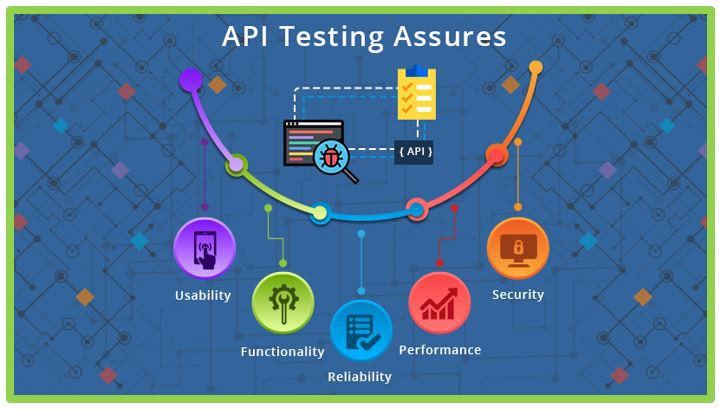
\includegraphics[width=5cm]{./img/1.png} 
\end{center}

Estos son algunos de los mayores beneficios de usar una herramienta de prueba de API, como se mencionó brevemente anteriormente.
\\•	Configuración y prueba más rápidas de los puntos finales (no tiene que pasar por todo el flujo de usuarios para configurar los datos y luego ejecutar los comandos para cambiar los datos),
\\•	Menor interacción en la línea de comandos,
\\•	Varias formas de configurar la autorización según el tipo que esté utilizando,
\\•	Mejor formato del código enviado y recibido,
\\•	Pruebas de rendimiento y confiabilidad más fáciles.
\\

\textbf{LOS CONTENDIENTES: POSTMAN E INSOMNIA}\\
Hay dos herramientas de prueba de API populares de las que hablaré hoy. Postman , un conjunto de herramientas que factura su ecosistema como:
\\"El único entorno de desarrollo de API completo" - Postman
\\E Insomnia , un cliente de REST que afirma que puedes
\\"Depurar API como un humano, no un robot" - Insomnia
\\

\textbf{BENEFICIOS DE INSOMNIA Y POSTMAN}\\
Insomnia y Postman comparten muchos beneficios que son extremadamente útiles para los desarrolladores de equipos de front-end, back-end y full-stack.
\\Ambos se jactan de:
\\•	Una versión gratuita de su software para los usuarios (actualizable a versiones pagas con más funciones en cualquier momento),
\\•	Al ser proyectos de código abierto,
\\•	Permitir múltiples espacios de trabajo (por ejemplo, desarrollo, aceptación, producción, etc.),
\\•	La capacidad de establecer el entorno y las variables locales estáticas que se actualizan con cada llamada a un punto final (a veces denominado encadenamiento de solicitudes).
\\•	Permitiendo la importación y exportación de datos de prueba para compartir fácilmente entre los miembros del equipo,
\\•	La capacidad de guardar llamadas y organizarlas en carpetas o colecciones,
\\•	Opciones de prueba e integración GraphQL,
\\•	Múltiples formas de configurar autorizaciones (OAuth, tokens de portador, Basic, HAWK, etc.) y generar / administrar cookies,
\\•	Y ambos tienen esquemas de colores claros y oscuros (sé que no es gran cosa, pero vale la pena señalarlo. Realmente prefiero desarrollar en un IDE oscuro a uno blanco).
\\Bien, ahora veamos algunas de las ofertas únicas de ambas herramientas.

\textbf{POSTMAN}\\
Estas son algunas de las cosas que distinguen a Postman de otras herramientas de prueba de API.
\\•	Documentación de API (Postman generará y alojará documentación de API basada en navegador en tiempo real),
\\•	Ejecuciones de colección (ejecutar un grupo de solicitudes como una serie en un entorno correspondiente; esto es muy útil para las pruebas automatizadas.
\\•	Monitorear dónde Postman ejecutará periódicamente una recopilación para verificar su rendimiento y respuesta,
\\•	Pruebas escritas en JavaScript simple que verificarán el objeto de respuesta, el tiempo, etc. desde el punto final,
\\•	Y servidores simulados para que los equipos simulen cada punto final y su respuesta correspondiente en una Colección Postman. Los desarrolladores pueden ver las respuestas potenciales, sin tener un back-end, y los miembros del equipo pueden alinearse con las expectativas durante las primeras fases del desarrollo de la API.
\\

\textbf{Ejemplo}


•Agregar Persona
\begin{center}
	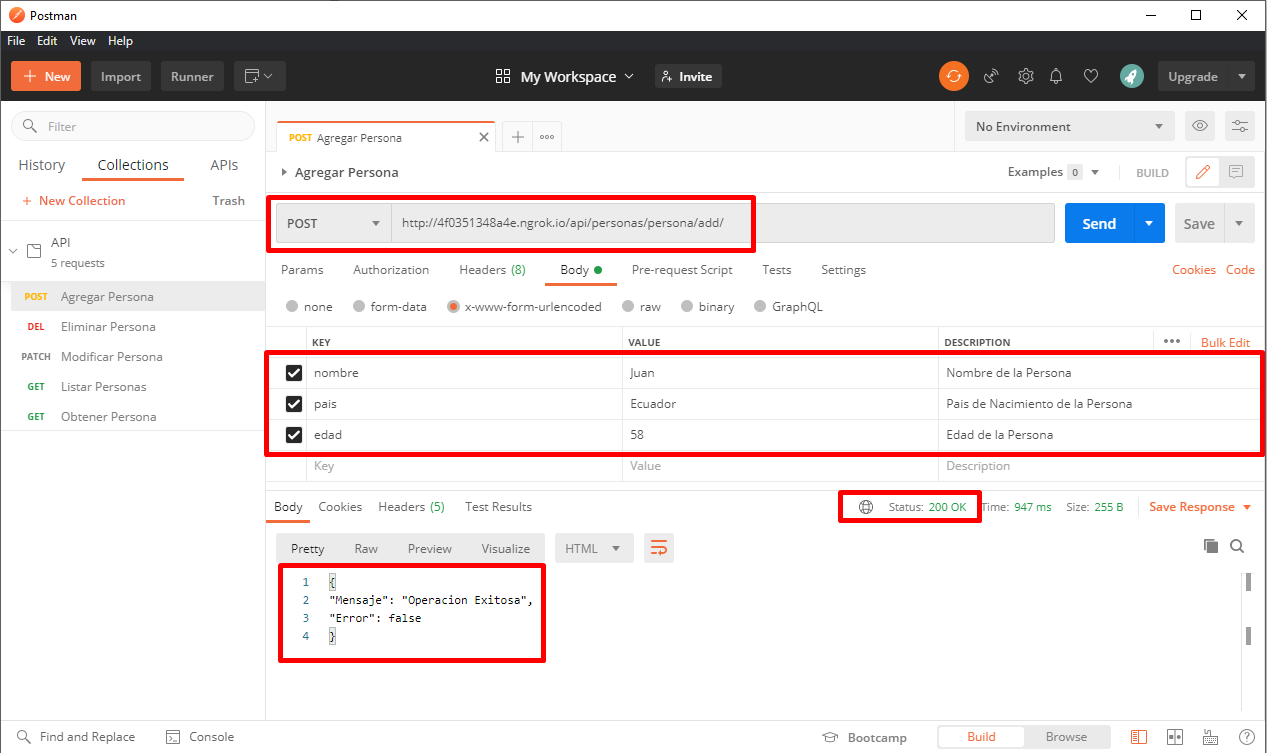
\includegraphics[width=5cm]{./img/3.png} 
\end{center}
 
\begin{center}
	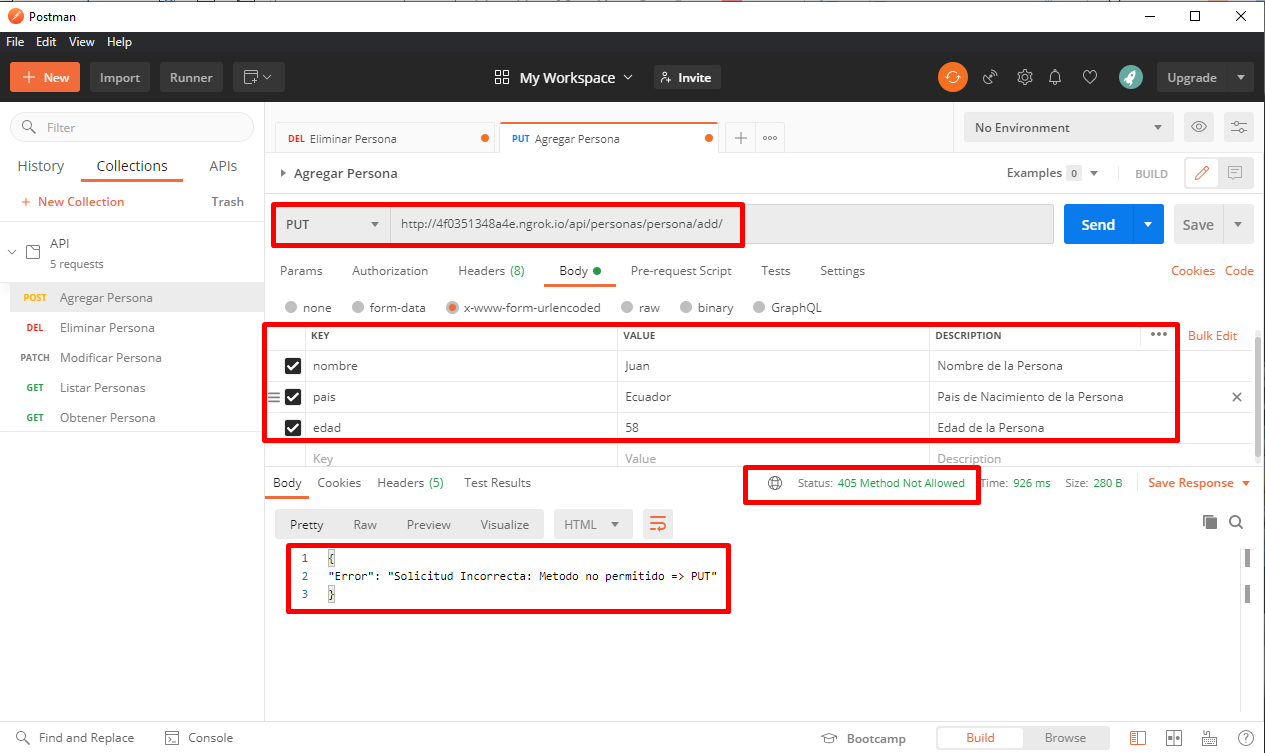
\includegraphics[width=5cm]{./img/4.png} 
\end{center}
 
•Eliminar Persona
\begin{center}
	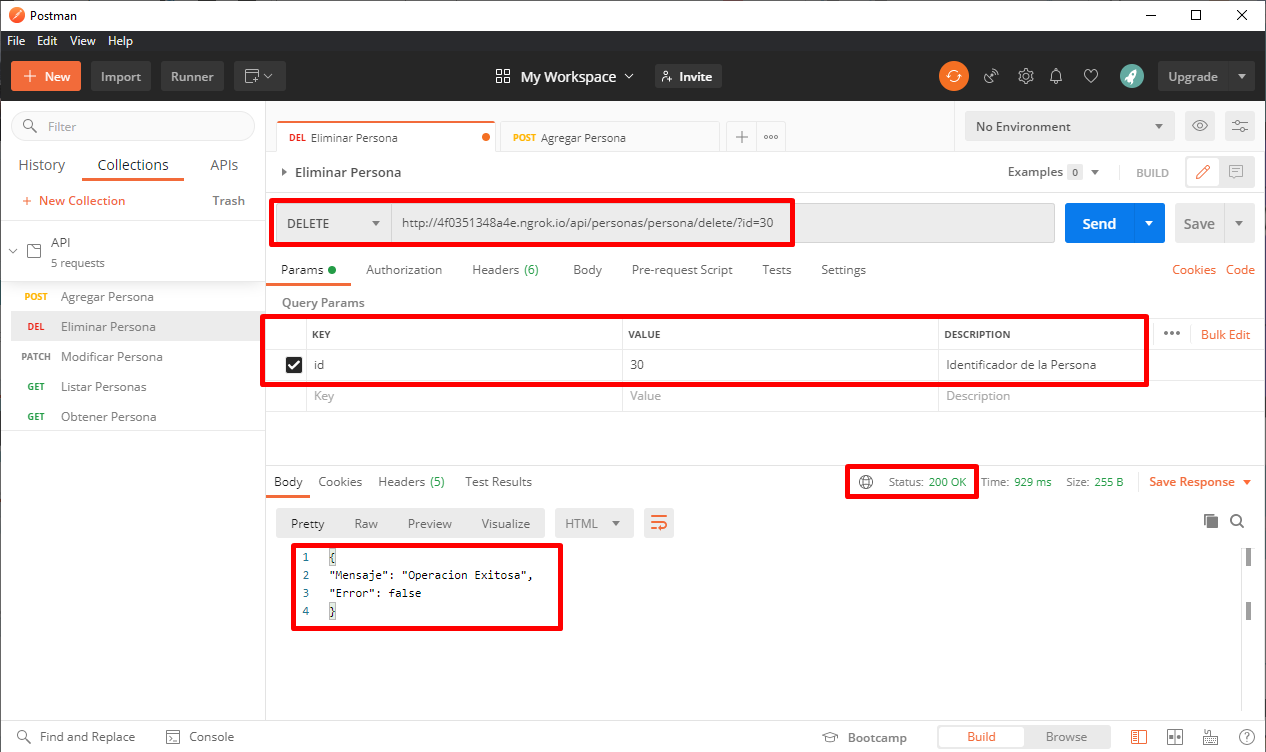
\includegraphics[width=5cm]{./img/5.png} 
\end{center}
\begin{center}
	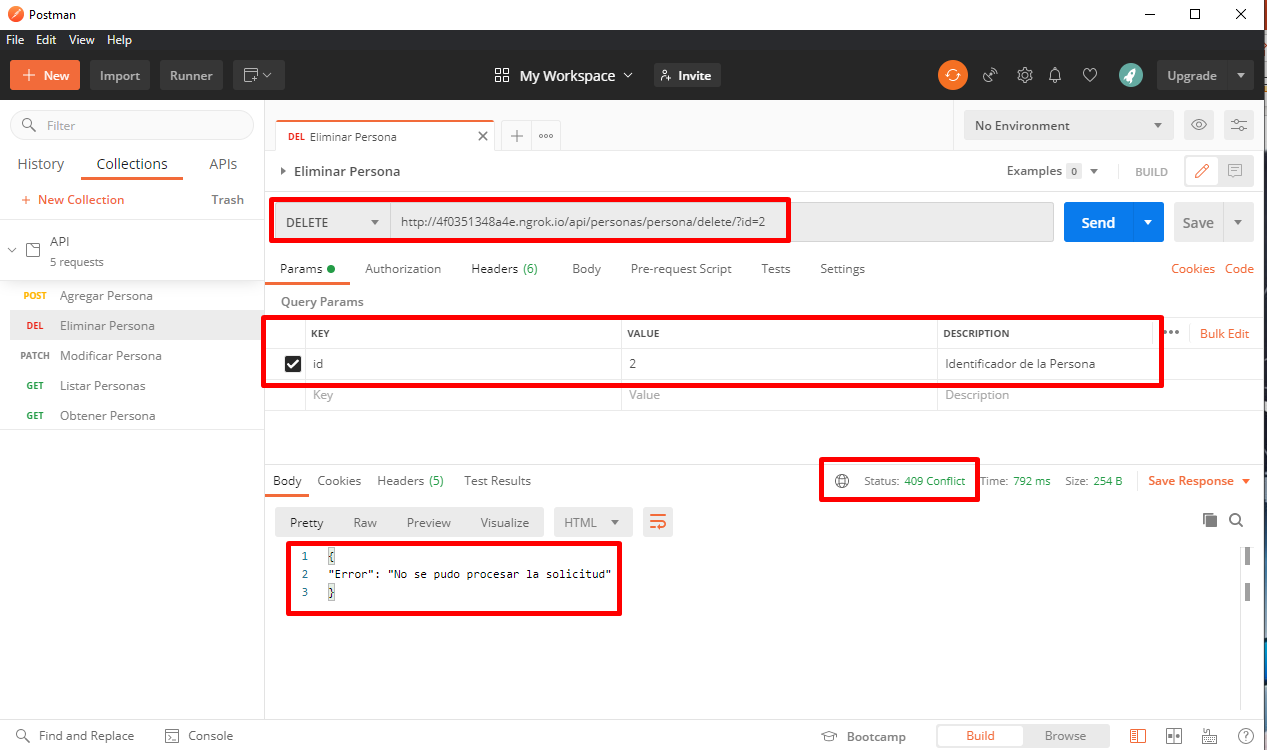
\includegraphics[width=5cm]{./img/6.png} 
\end{center}
 
 

•Modificar Persona
\begin{center}
	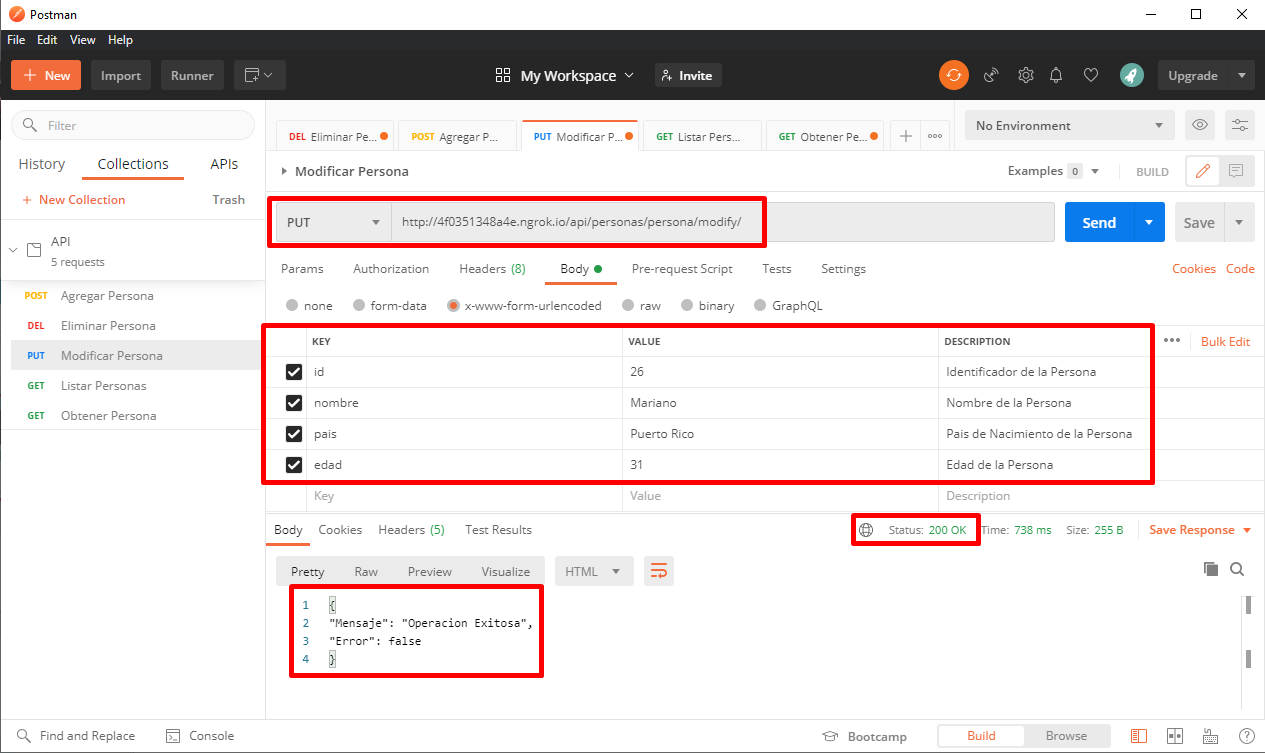
\includegraphics[width=5cm]{./img/7.png} 
\end{center}
\begin{center}
	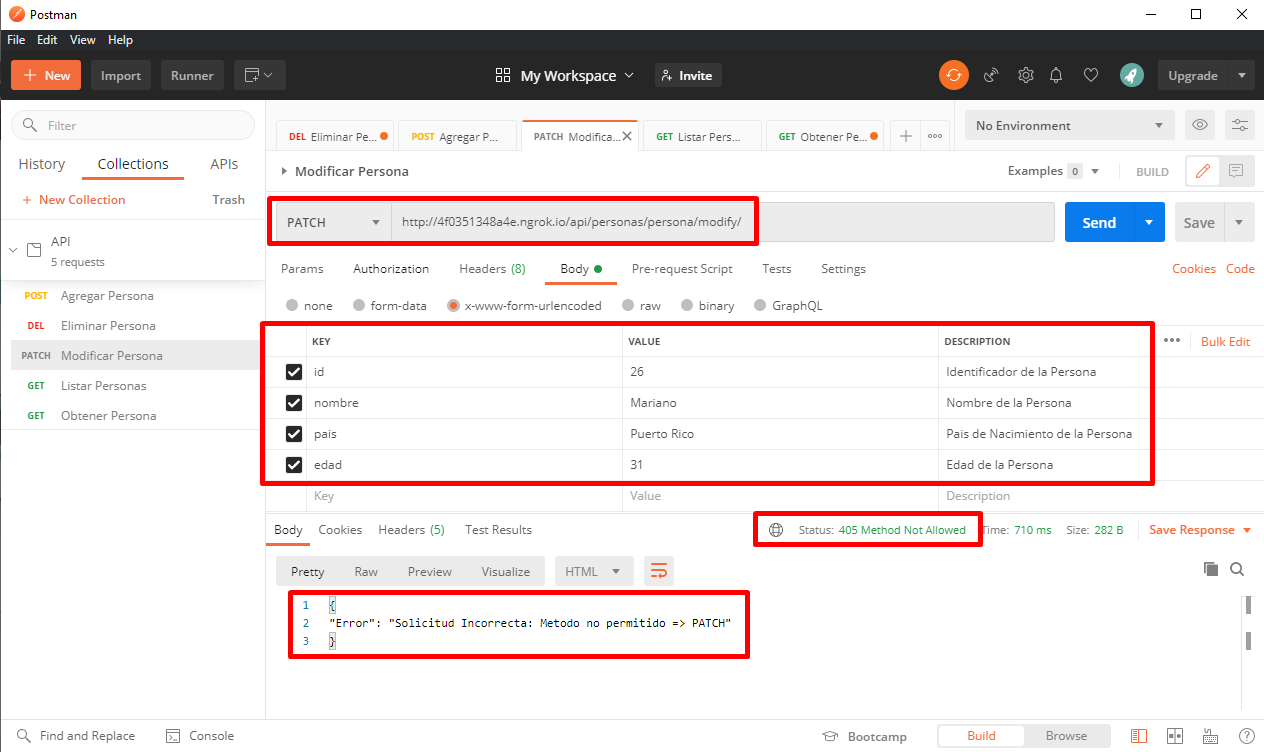
\includegraphics[width=5cm]{./img/8.png} 
\end{center}
 
 
•Listar Personas
\begin{center}
	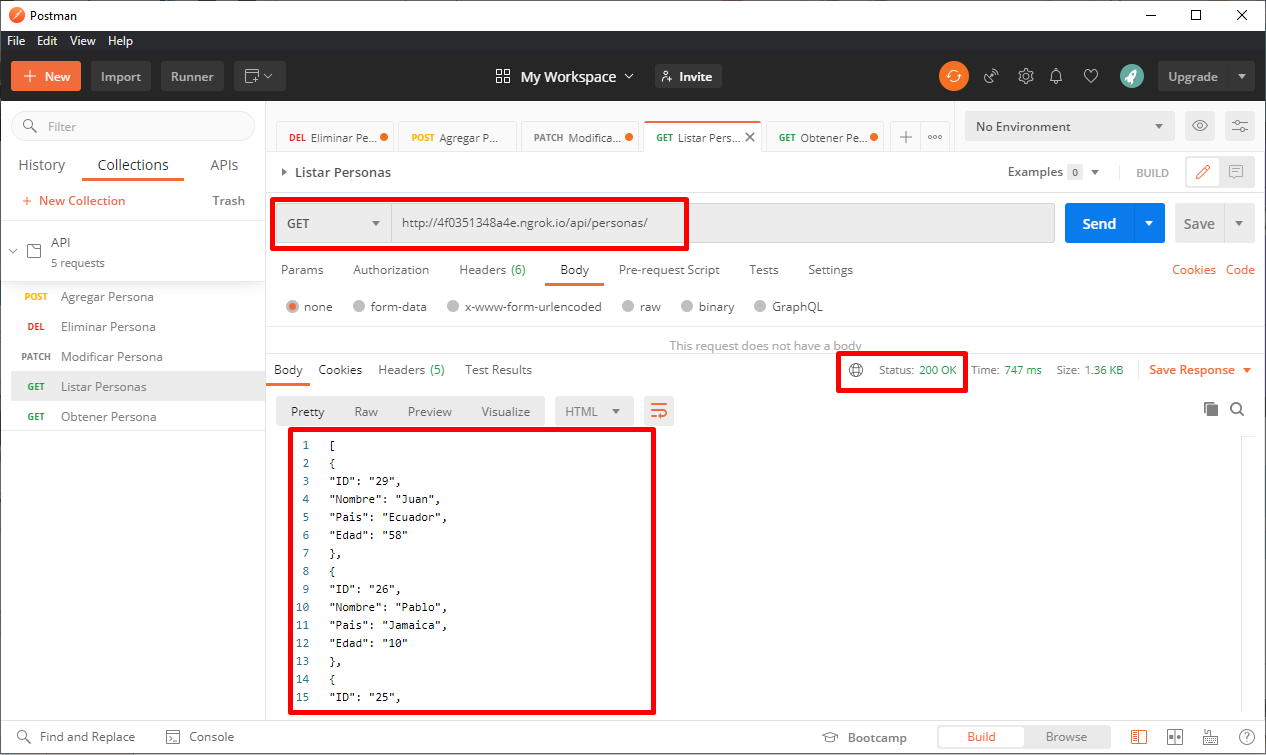
\includegraphics[width=5cm]{./img/9.png} 
\end{center}
 
•Obtener Persona

\begin{center}
	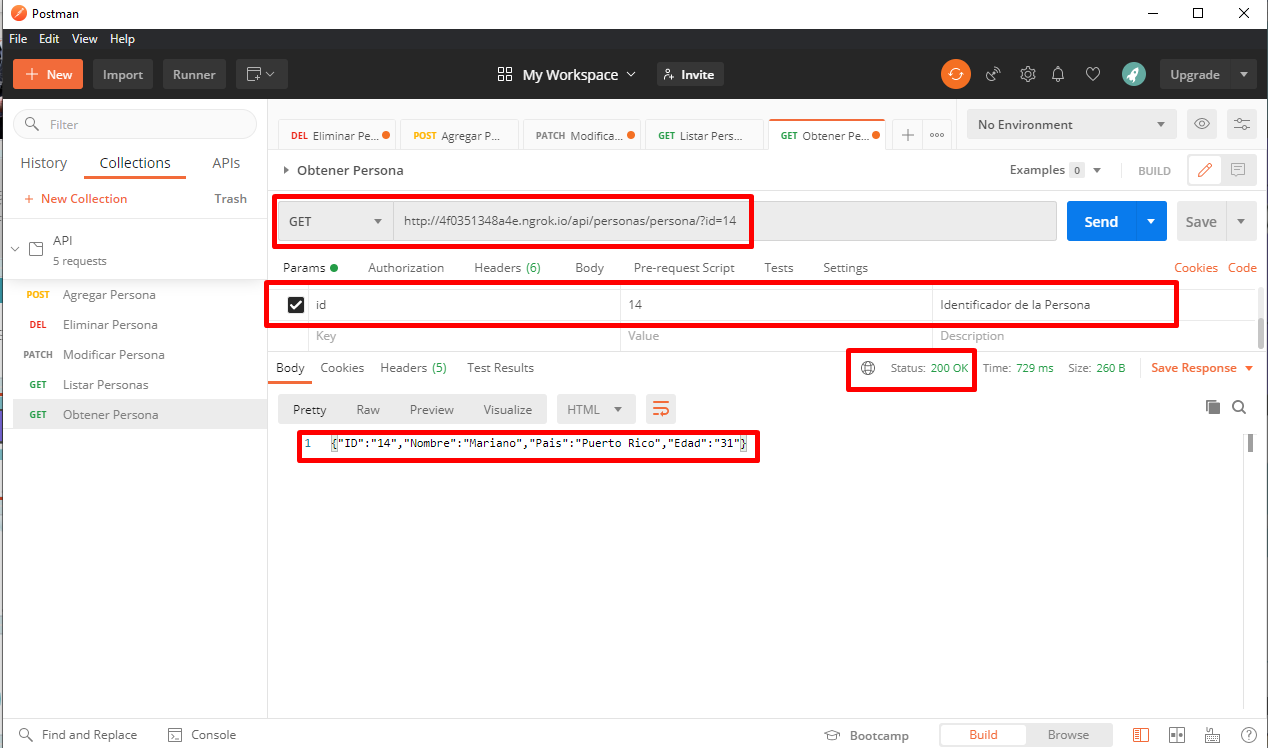
\includegraphics[width=5cm]{./img/10.png} 
\end{center}
\begin{center}
	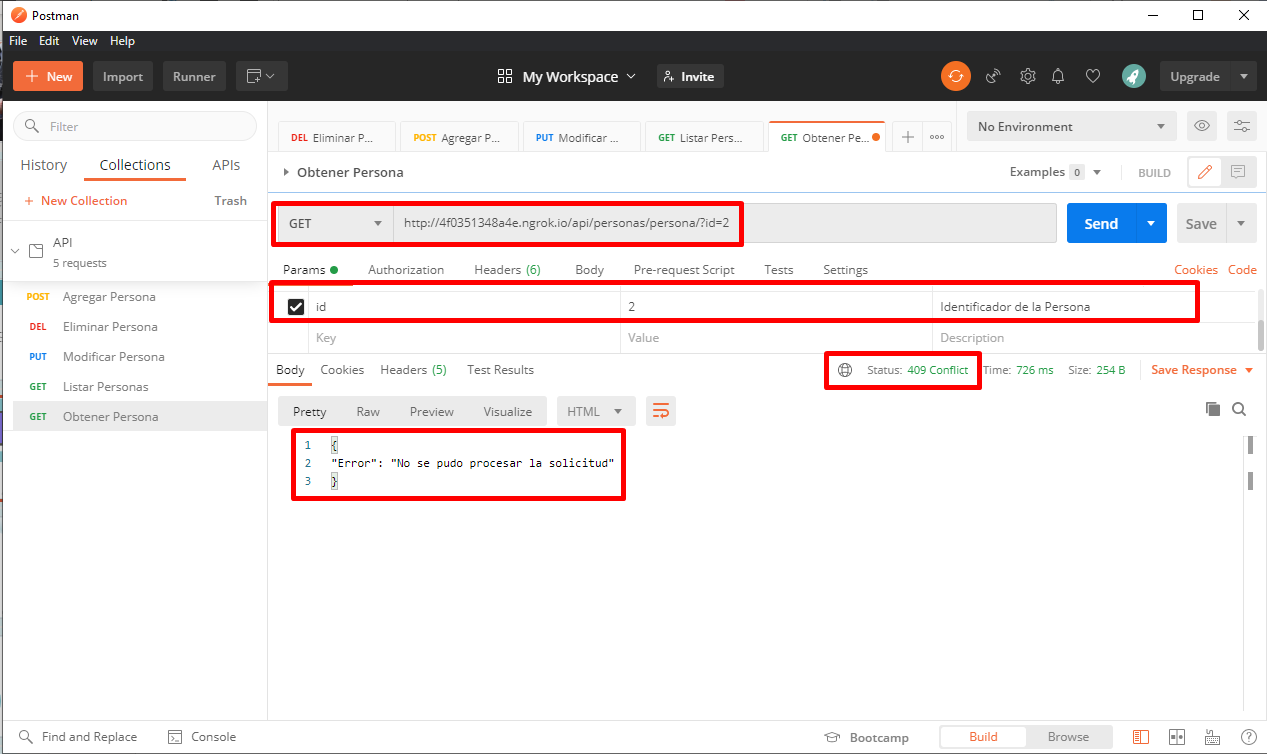
\includegraphics[width=5cm]{./img/11.png} 
\end{center}
 
\textbf{INSOMNIA}\\
\begin{center}
	
\includegraphics[width=5cm]{./img/12.png} 
\end{center}
Insomnia , en su defensa, tiene algunas cosas interesantes que ofrece que Postman no tiene.
\\•	Etiquetas de plantilla (similares a las variables de entorno, pero realizan operaciones en cosas como cadenas, marcas de tiempo, etc.),
\\•	La capacidad de crear nuevos complementos para Insomnia y su comunidad de usuarios,
\\•	Asignaciones de certificados de cliente a espacios de trabajo y validación SSL (o su desactivación),
\\•	Generación de fragmentos de código en 12 idiomas diferentes (útil si desea CURLAR el comando desde la línea de comando o colocarlo en su base de código real),
\\•	Un área de documentación muy completa donde se pueden agregar cosas como instrucciones, fragmentos de código e incluso datos de prueba a llamadas o colecciones específicas.
\\•	Visualización de la respuesta más allá de JSON y XML (con Insomnia puede ver páginas HTML, imágenes, SVG, archivos de audio e incluso documentos PDF).
\\•	Además, cosas útiles y prácticas a las que tener acceso al desarrollar API.
\\Ejemplo
\\•	Crear variables para las rutas
\begin{center}
	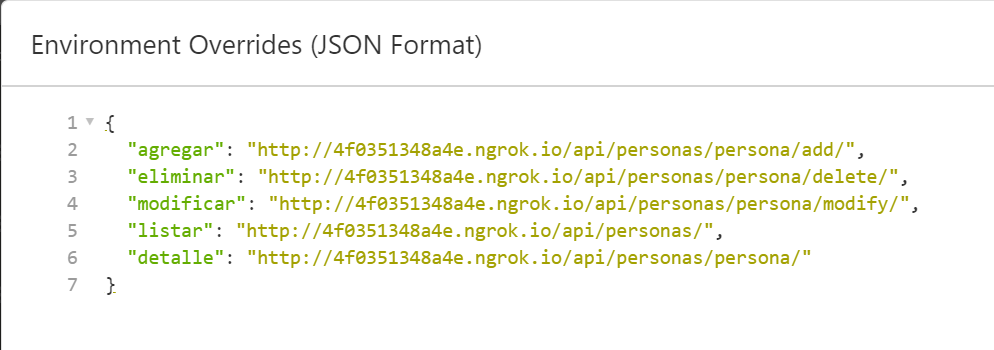
\includegraphics[width=5cm]{./img/13.png} 
\end{center}

•	Agregar Persona
\begin{center}
	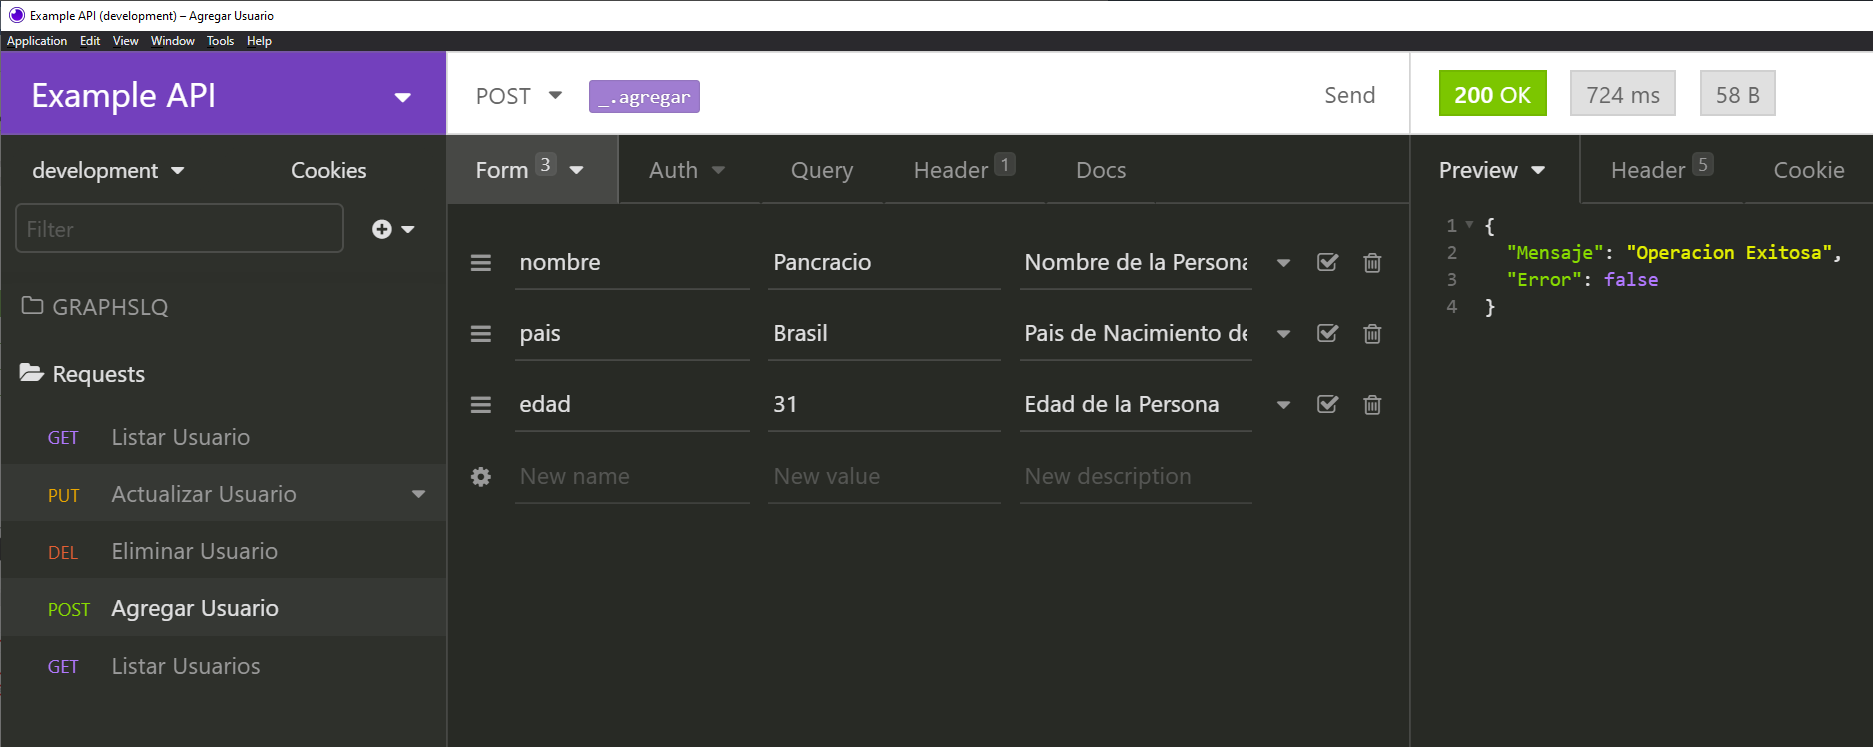
\includegraphics[width=5cm]{./img/14.png} 
\end{center}

•	Eliminar Persona
\begin{center}
	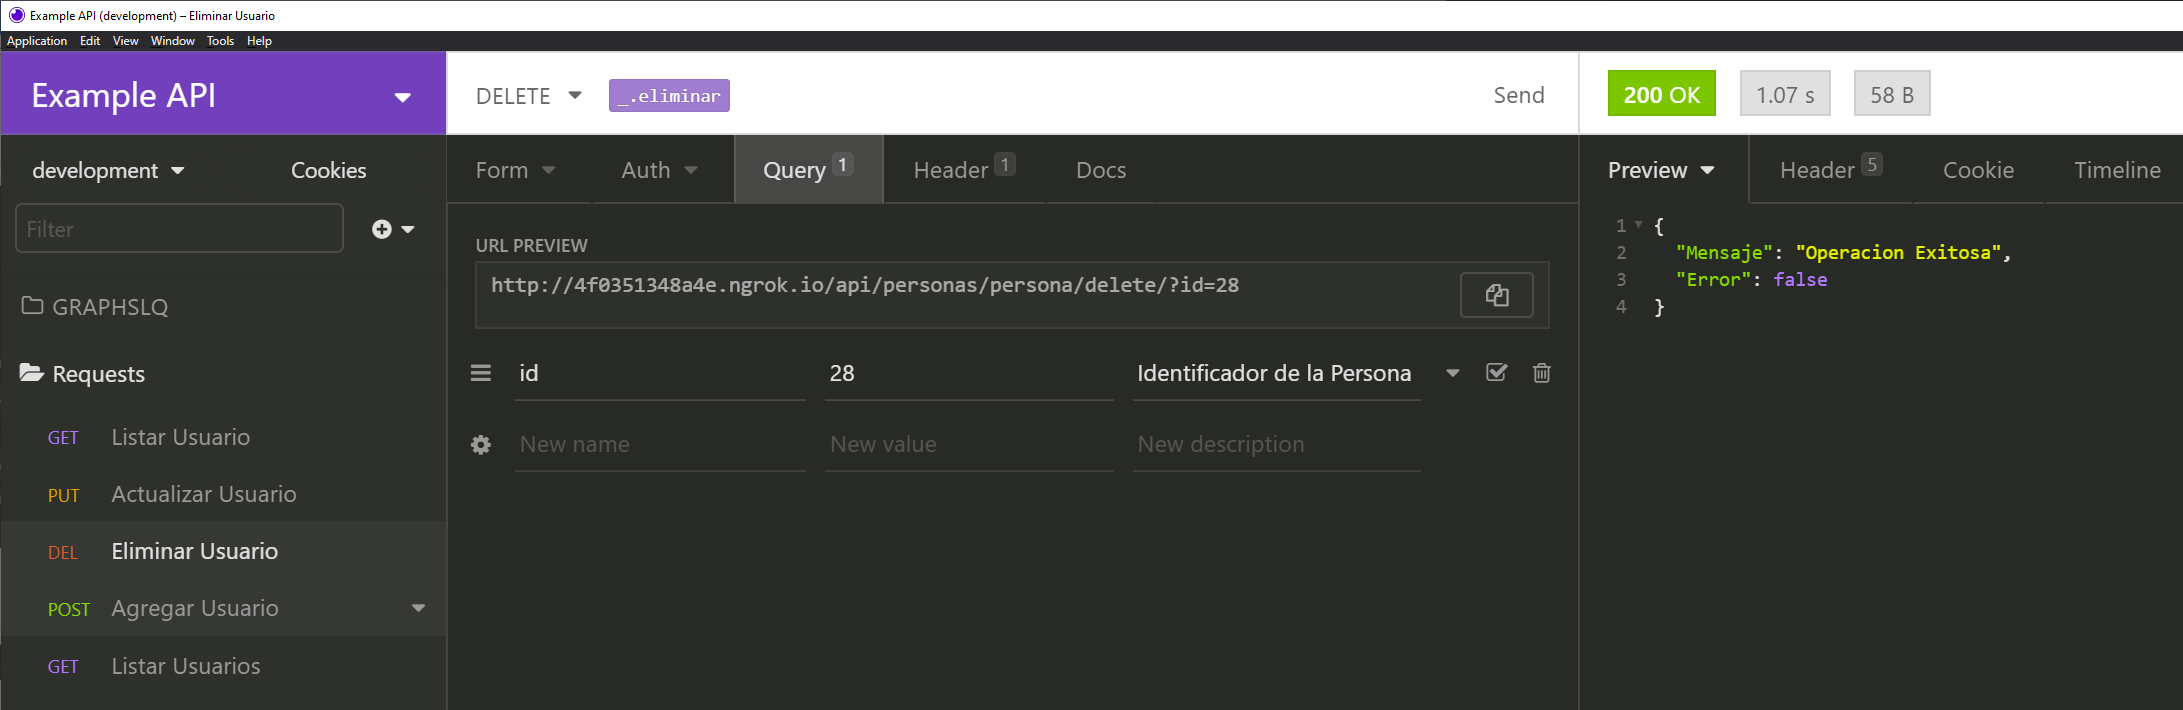
\includegraphics[width=5cm]{./img/15.png} 
\end{center}

•	Modificar Persona
\begin{center}
	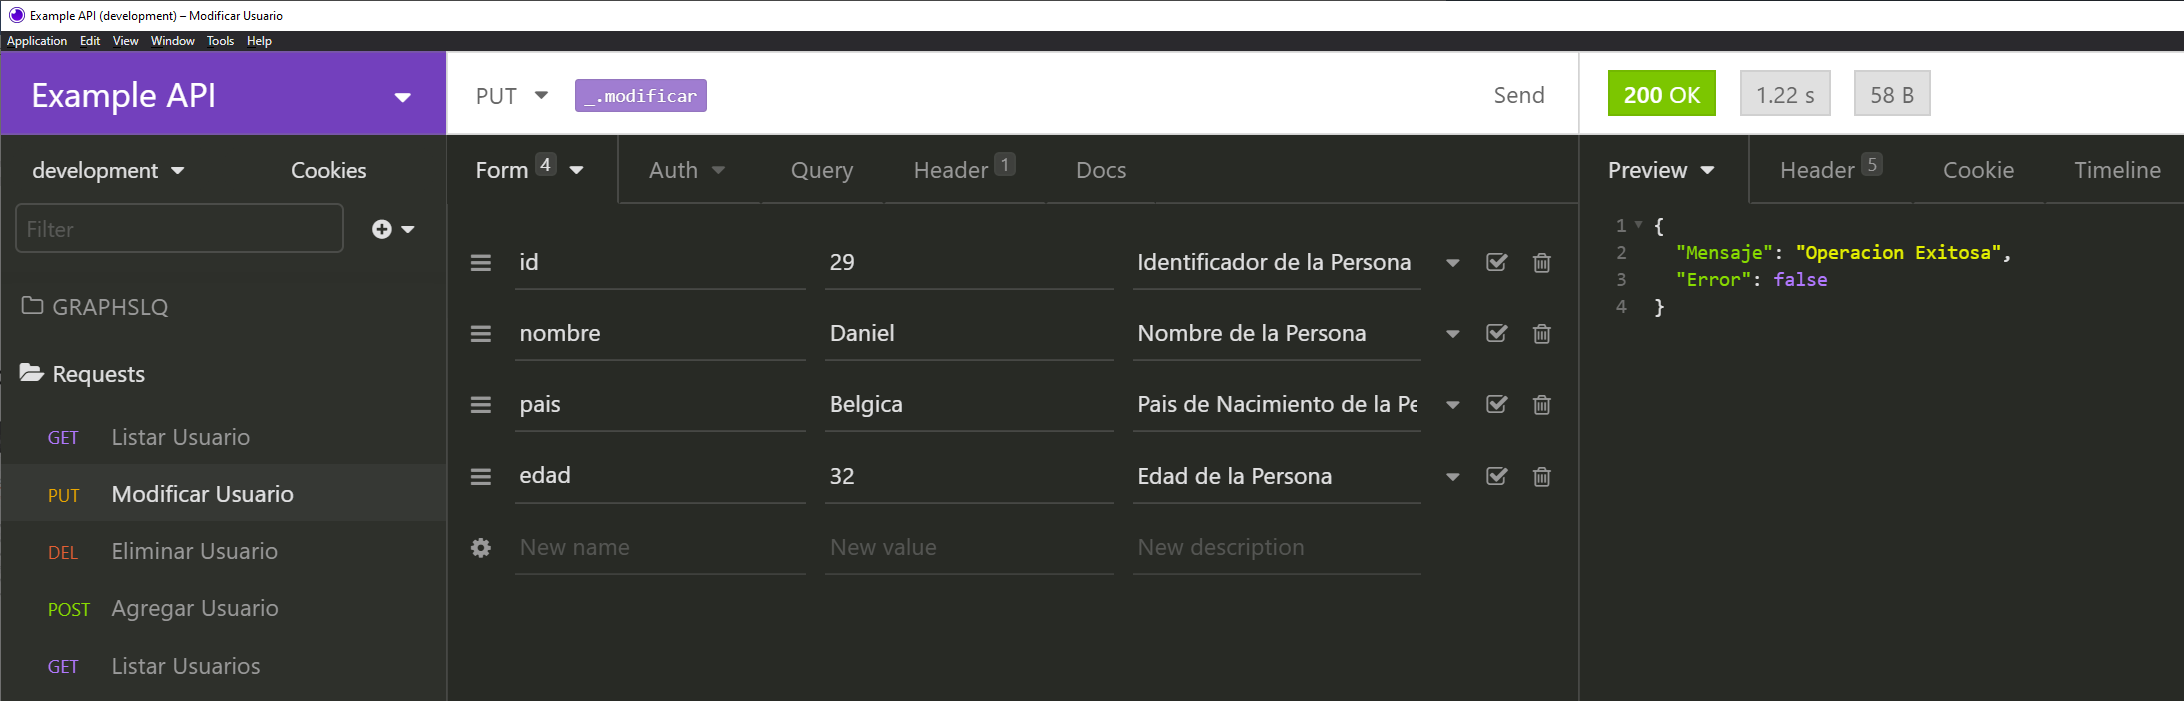
\includegraphics[width=5cm]{./img/16.png} 
\end{center}

•	Listar Persona
\begin{center}
	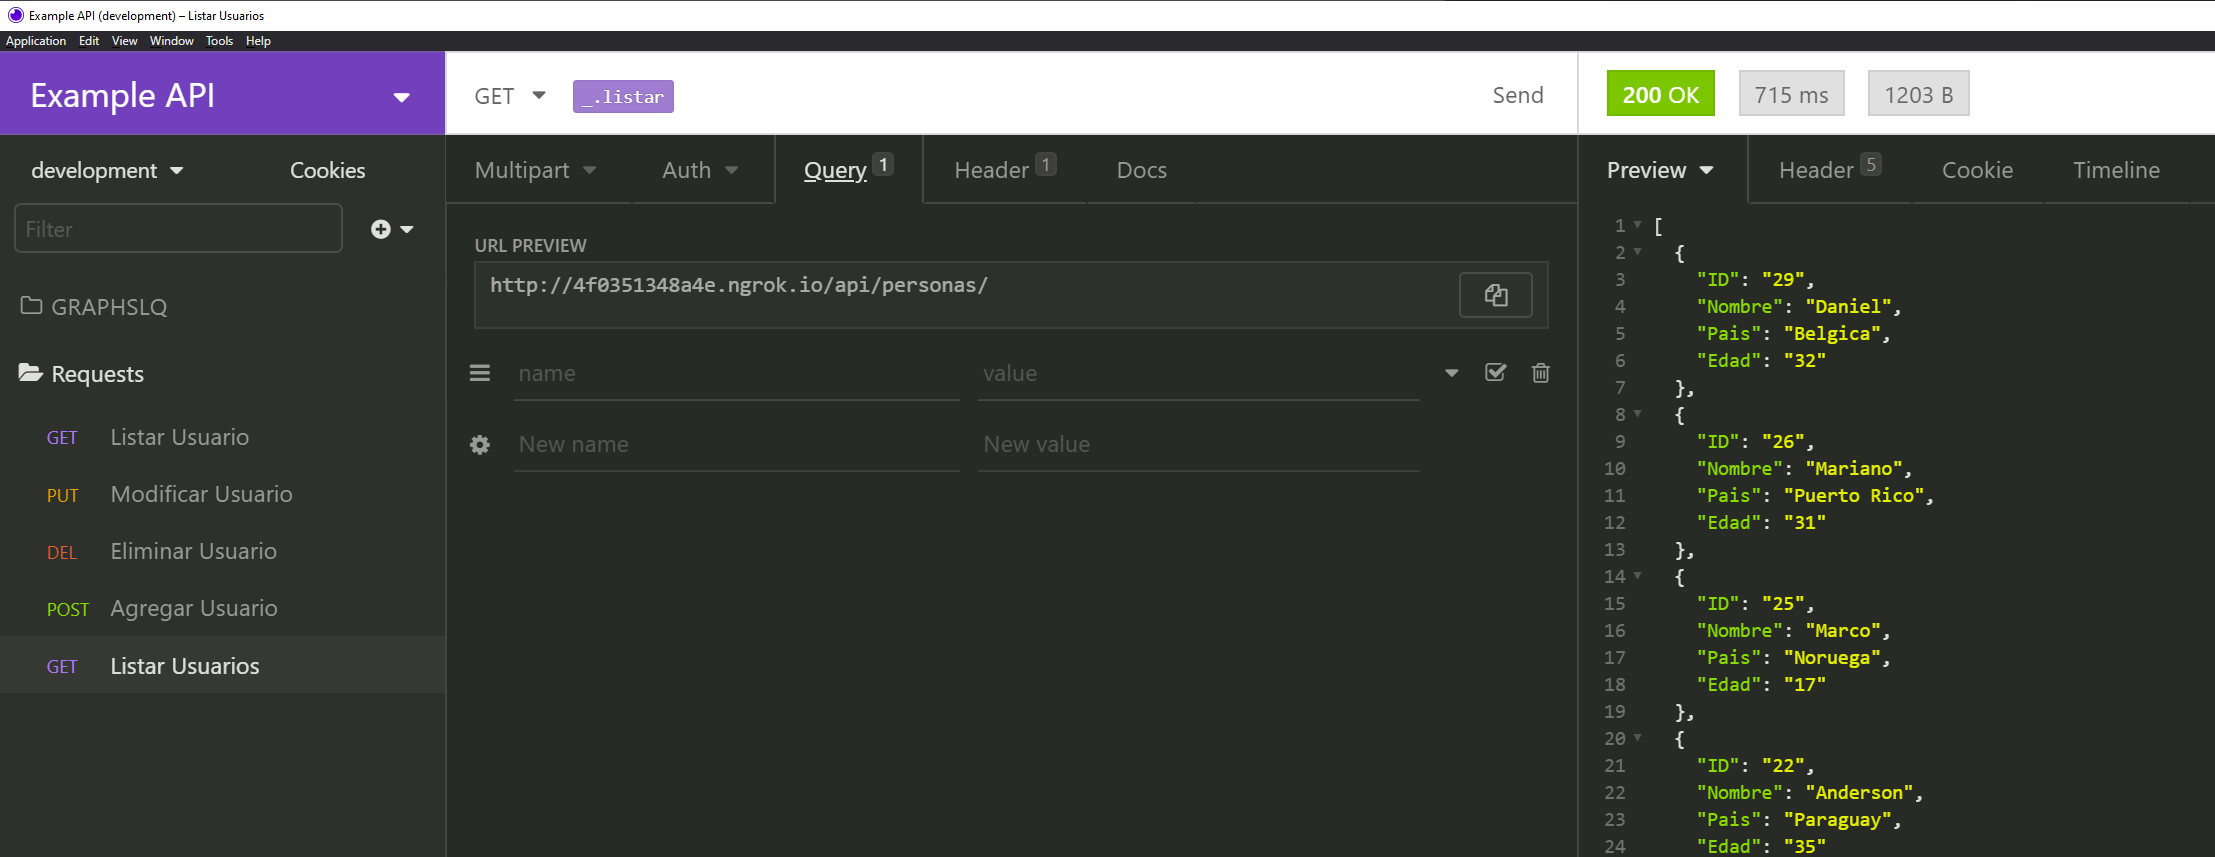
\includegraphics[width=5cm]{./img/17.png} 
\end{center}

•	Obtener Persona
\begin{center}
	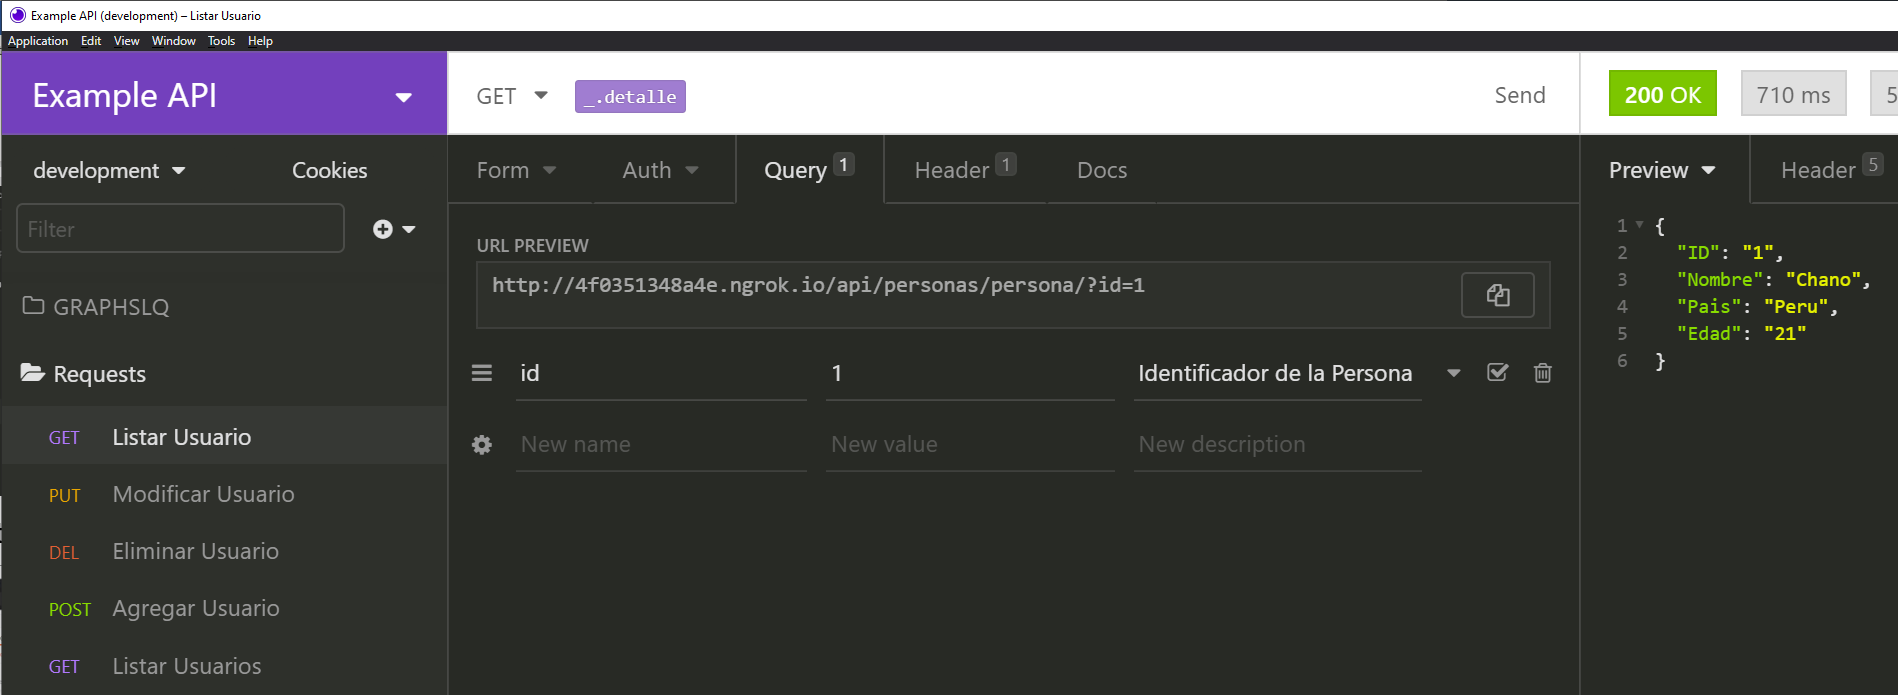
\includegraphics[width=5cm]{./img/18.png} 
\end{center}



\textbf{COMPARATIVA ENTRE POSTMAN E INSOMNIA}\\


\textbf{UX y rendimiento}\\

\begin{center}
	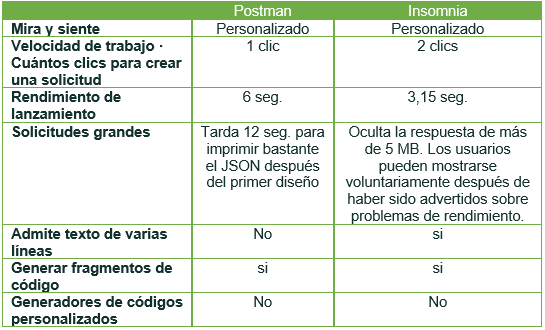
\includegraphics[width=5cm]{./img/19.png} 
\end{center}

\textbf{Mira y siente. } Postman e Insomnia tienen interfaces de usuario personalizadas y Insomnia parece más simple que Postman.
\\\textbf{Clics para crear una solicitud. }  Todos los proveedores obtuvieron resultados bastante bajos al crear una solicitud con solo un clic o dos.
\\\textbf{Velocidad de lanzamiento.  }  La apertura de las diferentes aplicaciones puede variar según su máquina. Sin embargo, Paw pudo abrirse en ~ 1.4 segundos, Postman registró alrededor de 6 segundos e Insomnia se lanzó en ~ 3.15 segundos.
\\\textbf{Manejo de grandes solicitudes.  }  Insomnia oculta respuestas de más de 5 MB y el usuario puede elegir ver la respuesta completa después de una advertencia de rendimiento. Postman muestran buenas velocidades con objetos de gran respuesta. A pesar de sus similitudes, Paw pudo cargar e "imprimir bastante" (formatear el JSON para que fuera más fácil de leer) un objeto de respuesta de 10 MB en menos de medio segundo.
\\\textbf{Admite texto de varias líneas.  }  Solo Insomnia admite texto de varias líneas.
\\\textbf{Genere fragmentos de código.  }  Todos los servicios permiten al usuario crear fragmentos de código para diferentes lenguajes de programación.


\textbf{Autenticación}\\

\begin{center}
	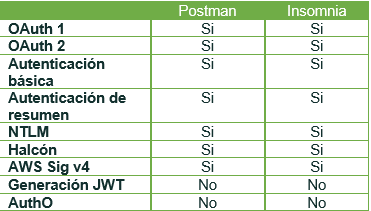
\includegraphics[width=5cm]{./img/20.png} 
\end{center}

Las opciones de autenticación fueron bastante consistentes en todos los ámbitos para los tres clientes API. Además de los mecanismos de autenticación admitidos desde el primer momento.
Al usar Postman, vale la pena señalar que la configuración de OAuth 2 no se almacena con la solicitud (solo se almacena el token). Por lo tanto, si el usuario desea recuperar el token nuevamente, debe ingresar todos los parámetros de OAuth por segunda vez.
\\


\textbf{Ambientes}\\

\begin{center}
	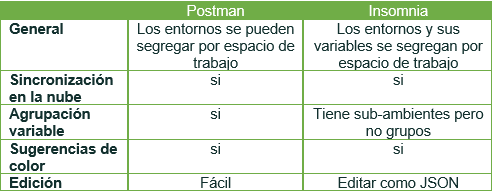
\includegraphics[width=5cm]{./img/21.png} 
\end{center}
Cuando se trabaja con clientes de API, normalmente es necesario crear variables de entorno que ayuden con las pruebas y simulaciones de API. Además, las variables de entorno se pueden utilizar para configuraciones como el manejo de cookies o encabezados. Los detalles se vuelven aún más importantes cuando se maneja la seguridad. Es bueno poder separar las variables de entorno entre las API porque algunas API tienen muchas variables adjuntas en el cliente.\\
\\\textbf{General. } Todos los servicios soportan entornos. Además, Insomnia  permiten al usuario segregar variables de entorno por proyecto (espacio de trabajo). En Postman, la agrupación de variables se denomina entornos que se pueden compartir entre espacios de trabajo.
\\Insomnia permite al usuario crear sub-entornos con fines de organización.
\\\textbf{Sincronización en la nube. }  Insomnia y Postman proporcionan capacidades de sincronización.
\\\textbf{Editando entornos.  }  Postman tienen una vista de tabla intuitiva para editar variables. Puede editar las variables de Insomnia en un componente de entrada JSON.

\textbf{Descripción API}\\

\begin{center}
	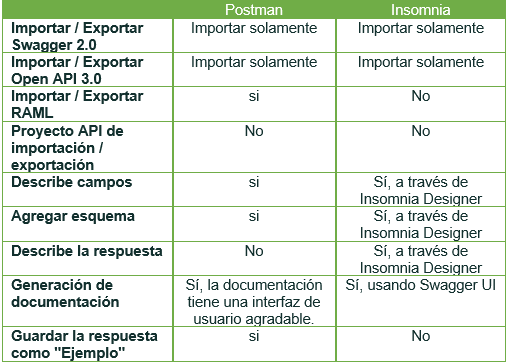
\includegraphics[width=5cm]{./img/22.png} 
\end{center}

La capacidad de describir y especificar fácilmente una API es enorme para el diseño de API. Por lo tanto, es muy importante que este proceso sea lógico y fácil para los desarrolladores. Muchas API buscan utilizar especificaciones como OpenAPI y Swagger. Estas especificaciones se pueden importar, exportar y generar en clientes API. Arriba hay una tabla que compara los servicios y lo que respaldan.

\textbf{Pruebas}\\


\begin{center}
	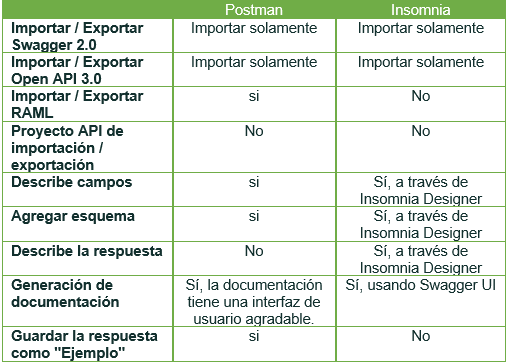
\includegraphics[width=5cm]{./img/22.png} 
\end{center}

La mayoría del software necesita algún tipo de prueba. Los clientes de API se pueden utilizar para ayudar a probar otras aplicaciones y software mediante el envío de solicitudes HTTP simuladas. Algunos servicios ofrecen pruebas dentro de su aplicación. De los dos clientes API de este artículo, Postman es el único que tiene capacidades de prueba.

\textbf{Precios}\\


A continuación se muestran los precios de los tres servicios según los planes ofrecidos. Postman e Insomnia ofrecen un nivel gratuito. Sin embargo, si planea seguir con el desarrollo y diseño de API.
\\Los usuarios y equipos más avanzados deben analizar más detenidamente las funciones por las que van a pagar.

\begin{center}
	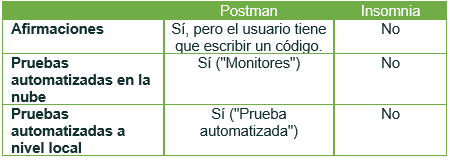
\includegraphics[width=5cm]{./img/23.png} 
\end{center}



\section{Conclusiones}
En general, tengo que decir que Postman aparece como el líder actual en términos de herramientas de prueba de API, en mi opinión. Es más maduro y con todas las funciones que Insomnia, y ofrece muchos beneficios realmente excelentes para los desarrolladores, incluso en su nivel gratuito.
Para mis equipos, que practican pruebas e implementaciones de CI / CD totalmente automatizadas, tener un corredor de colección de pruebas como Postman ofrece es un gran punto de venta, y si está completamente dedicado a respaldar una API, haber generado documentación en tiempo real también podría será muy agradable tenerlo.
Dicho esto, si Insomnia incorpora algunos de los beneficios de Postman a medida que continúa desarrollándose y mejorando, no hay razón para que no pueda seguir siendo un competidor muy fuerte en el mundo de las pruebas API.

\section{Recomendaciones}
Insomnia incorpora algunos de los beneficios de Postman a medida que continúa desarrollándose y mejorando, no hay razón para que no pueda seguir siendo un competidor muy fuerte en el mundo de las pruebas API.

\section{Biblografia}

\begin{itemize}
    \item Sharma, A. (2020). Automated API Testing with Postman. 
    Recuperado de https://www.c-sharpcorner.com/article/automated-api-testing-with-postman/    
    \item Paradigma Digital (2020). Postman: gestiona y construye tus APIs rápidamente.
    Recuperado de  https://www.paradigmadigital.com/dev/\\postman-gestiona-construye-tus-apis-rapidamente/    
    \item Smashing Magazine. (2020). How To Automate API Testing With Postman.
    Recuperado de https://www.smashingmagazine.com/20\\20/09/automate-api-testing-postman/    
    \item Retz, J. (2020). Insomnia vs Postman vs Paw: Comparing the Top API Clients.
    Recuperado de https://rapidapi.com/blog/insomnia-vs-postman-vs-paw/    
    \item Macknioght, K. (2020). How to use Insomnia to Test API Endpoints.
    Recuperado de  https://dev.to/kmcknight91/how-to-use-insomnia-to-test-api-endpoints-1lad    
    \item Damrongchai, A. (2020). Test your APIs with Insomnia REST client.
    Recuperado de  https://medium.com/@artiwarahdamron\\gchai/test-your-apis-with-insomnia-rest-client-355093f32755    
    \item Brightest. (2020). Insomnia, not just another API client - Brightest.
    Recuperado de https://www.brightest.be/test-automation/insomnia-not-just-another-api-client/    
     \item Kedrosky, E., Clark, M., \& Gardner, R. (2020). Getting Started API Penetration Testing with Insomnia.
     Recuperado de https://securityboulevard.com/2020/04/\\getting-started-api-penetration-testing-with-insomnia/
     
\end{itemize}

%%%%%%%%%%%%%%%%%%%%%%%%%%%%%%%%%%%%%%%%%%%%%%%%%%%%%%%%%
\end{document}